%!TEX encoding = UTF-8 Unicode
\documentclass[12pt]{article} 
\usepackage[left=0.75in,top=20mm,right=0.75in,bottom=0.3in]{geometry} % Document margins
\usepackage{CJK}
\usepackage{graphicx}
\usepackage{mathtools}
\usepackage{mathrsfs}
\usepackage{amssymb}
\usepackage{hyperref}
\usepackage{sidecap}
\usepackage{makecell}
\usepackage{fancyhdr}

\fancypagestyle{title}{
  \setlength{\headheight}{15pt}
  \fancyhf{}
  \renewcommand{\headrulewidth}{0pt}
  \renewcommand{\footrulewidth}{0pt}
  \fancyhead[R]{Parallel Programming 2015}
}

\pagestyle{title}

\makeatletter
\renewenvironment{itemize}
{\list{$\bullet$}{\leftmargin\z@ \labelwidth\z@ \itemindent-\leftmargin
\let\makelabel\descriptionlabel}}
{\endlist}
\makeatother

\begin{CJK}{UTF8}{bsmi}
\title{\textbf{ Homework 2 /  Single Roller Coaster and NBody Simulation }}
\author{\textbf{李豪韋 (HW-Lee) ID 103061527}}
\date{}

\begin{document}
\vspace*{-60pt}
{\let\newpage\relax\maketitle}
\thispagestyle{title}

\vspace{-50pt}
\section*{Overview}
\vspace{-20pt}
\noindent\makebox[\linewidth]{\rule{\textwidth}{0.4pt}}
\vspace{5pt}

The project is aimed at helping us to get familiar with using Pthread and OpenMP, and it consists of two parts, namly single roller coaster simulation and NBody simulation. In single roller coaster simulation section, we are going to simulate real situations of a roller coaster and a couple of passengers by launching the same number of threads where each thread stands for a passenger. Each passenger will take a walk around the park for a random time and return back for another ride repeatly, and the roller coaster commences to run immediately when the number of people reaches the maximum that it can accommodate. In n-body section, we are going to simulate real moving of several bodies by calculating the force at each body at each iteration. There are two ways calculating the force, directly going through all bodies then summing up gravitational vectors of all pairs and Barnes-Hut algorithm.

\section*{Implementation}
\vspace{-20pt}
\noindent\makebox[\linewidth]{\rule{\textwidth}{0.4pt}}

\begin{enumerate}
	\item Single Roller Coaster Simulation
	\begin{flushleft}
		Each passenger uses one independent thread such that there is no interaction between two passengers, and all threads use the same API, \texttt{rolcoaster->get\_in( passenger )}, which is surrounded by critical section, \texttt{mutex\_lock}/\texttt{mutex\_unlock}, to guarantee the API will not be driven by more than one thread simultaneously.
	\end{flushleft}

	\item NBody Simulation
	\begin{itemize}
		\item Normal
		\begin{flushleft}
			The set of bodies is simply separated into $n$ parts, where $n$ stands for the number of threads we can use, then computing and updating next velocity value of each body. After updating all velocity values of bodies, each thread starts to update next position of each body and finish an iteration. The reason why each thread updates bodies' position after all bodies' velocity has been updated is to avoid synchronization issues: if a body is moved, all the gravitational force will change as well and the results might be inaccurate.
		\end{flushleft}
		\item Barnes-Hut Algorithm
		\begin{flushleft}
			We know the root will have four children if the number of bodies is more then four. Note that in my case, that a node has no body inside is allowed and the node can be regarded as a zero-mass body. To reduce the time building BH-Tree, I simply parallelize the recursive process at the second layer: if the number of threads is greater than four, it still utilizes only four threads building the tree. Similarly, the set of bodies will be separated for each thread and the iteration will be executed in the same way as the way used in normal version.
		\end{flushleft}
	\end{itemize}
\end{enumerate}

\newpage

\section*{Analysis \& Results}
\vspace{-20pt}
\noindent\makebox[\linewidth]{\rule{\textwidth}{0.4pt}}

\begin{enumerate}
	\item Single Roller Coaster Simulation
	\begin{figure}[ht]
		\hspace{-20pt}
		\begin{minipage}{.48\textwidth}
			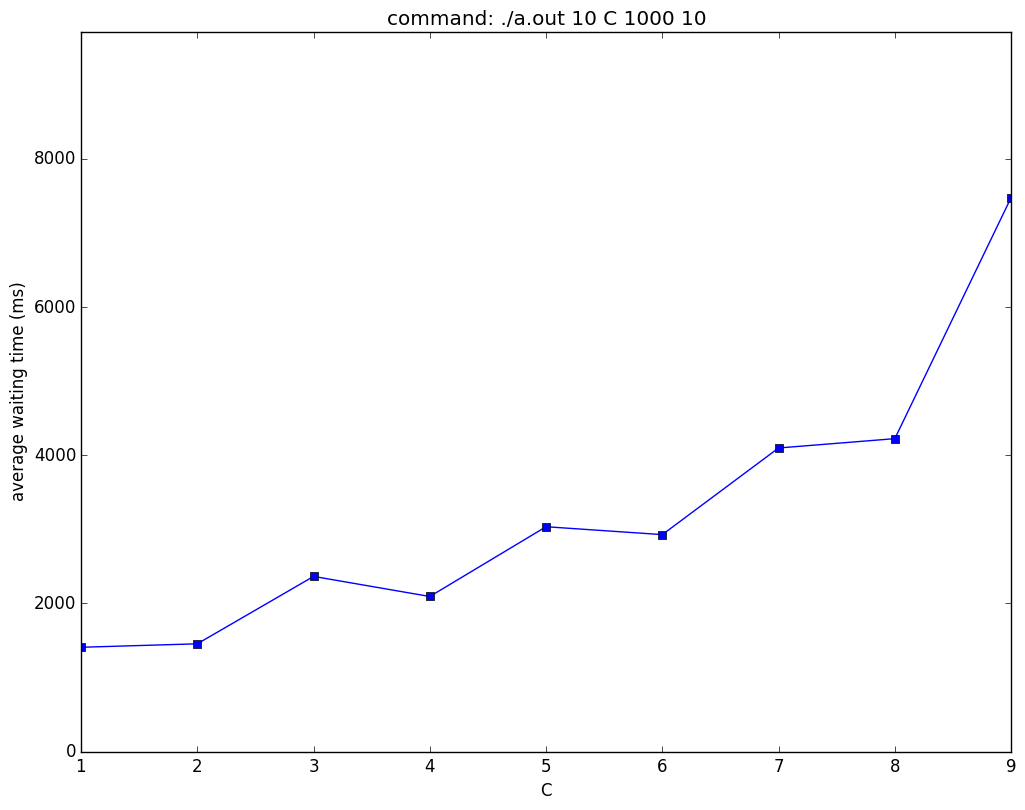
\includegraphics[scale=.35]{./SRCC_C.png}
			\caption{Average waiting time with different values of capacity}
		\end{minipage}
		\hspace{40pt}
		\begin{minipage}{.48\textwidth}
			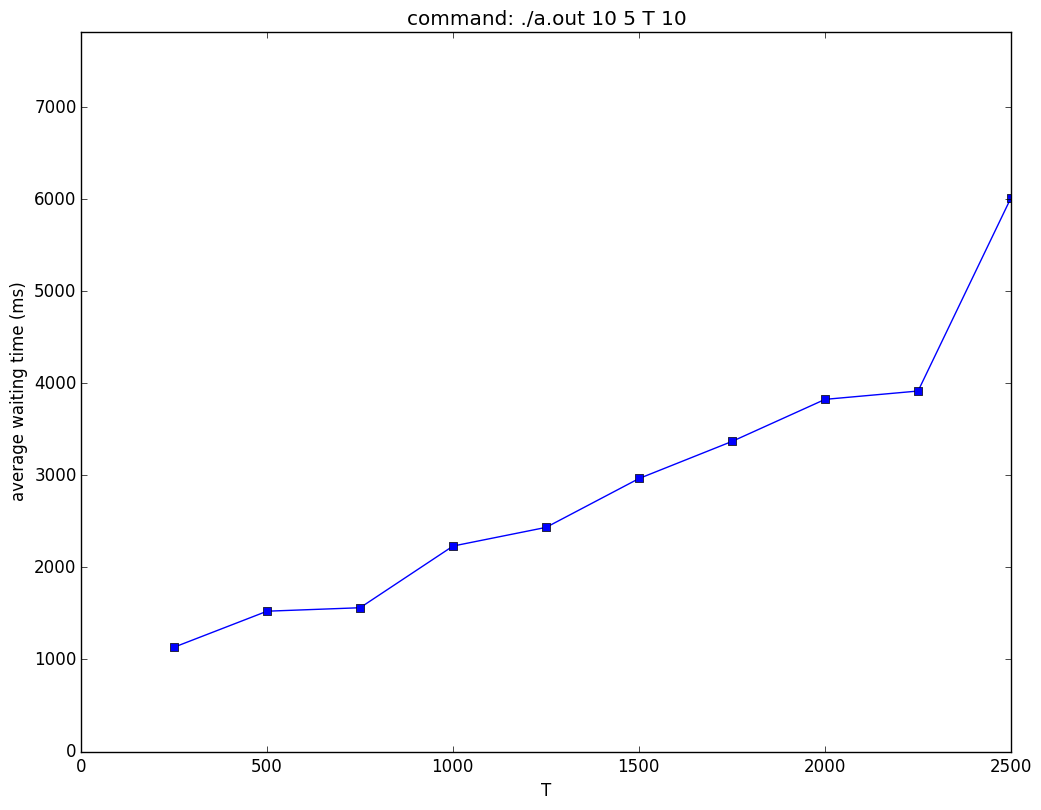
\includegraphics[scale=.35]{./SRCC_T.png}
			\caption{Average waiting time with different period of a track}
		\end{minipage}
	\end{figure}

	\item NBody Simulation
	\begin{itemize}
		\item Partition
		\begin{SCfigure}[][h]
			\vspace{-20pt}
			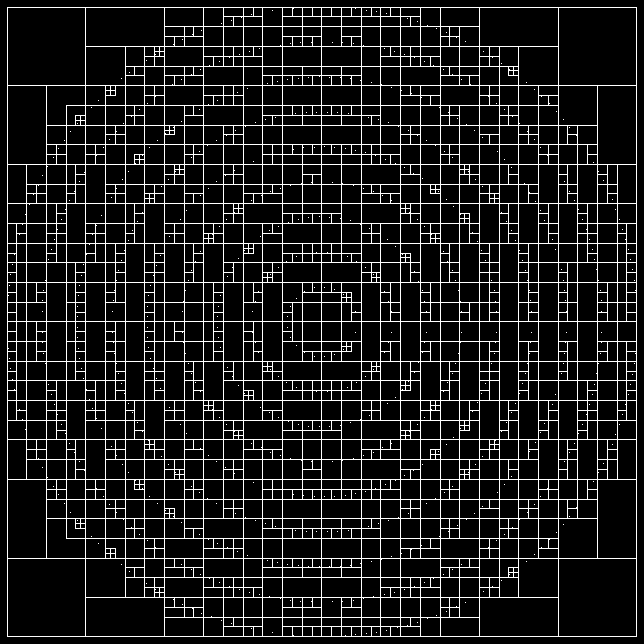
\includegraphics[scale=.45]{./partition.png}
			\caption{Visual result example after building tree: the set of bodies will be divided into four clusters recursively until each smallest cluster has less than or equal to one body}
		\end{SCfigure}

		\newpage

		\item Computation time with various implementations
		\begin{center}
			\begin{SCfigure}[][h]
				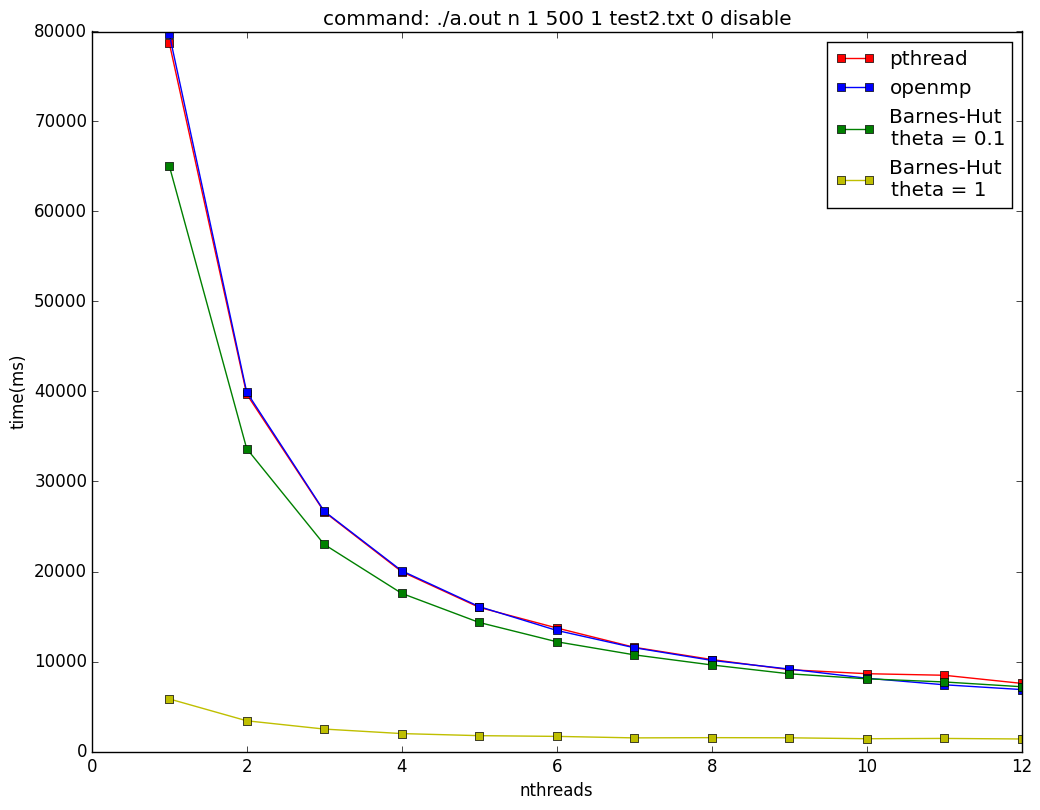
\includegraphics[scale=.5]{./nthreads.png}
				\caption{Results with different number of threads}
			\end{SCfigure}

			\begin{SCfigure}[][h]
				\vspace{-80pt}
				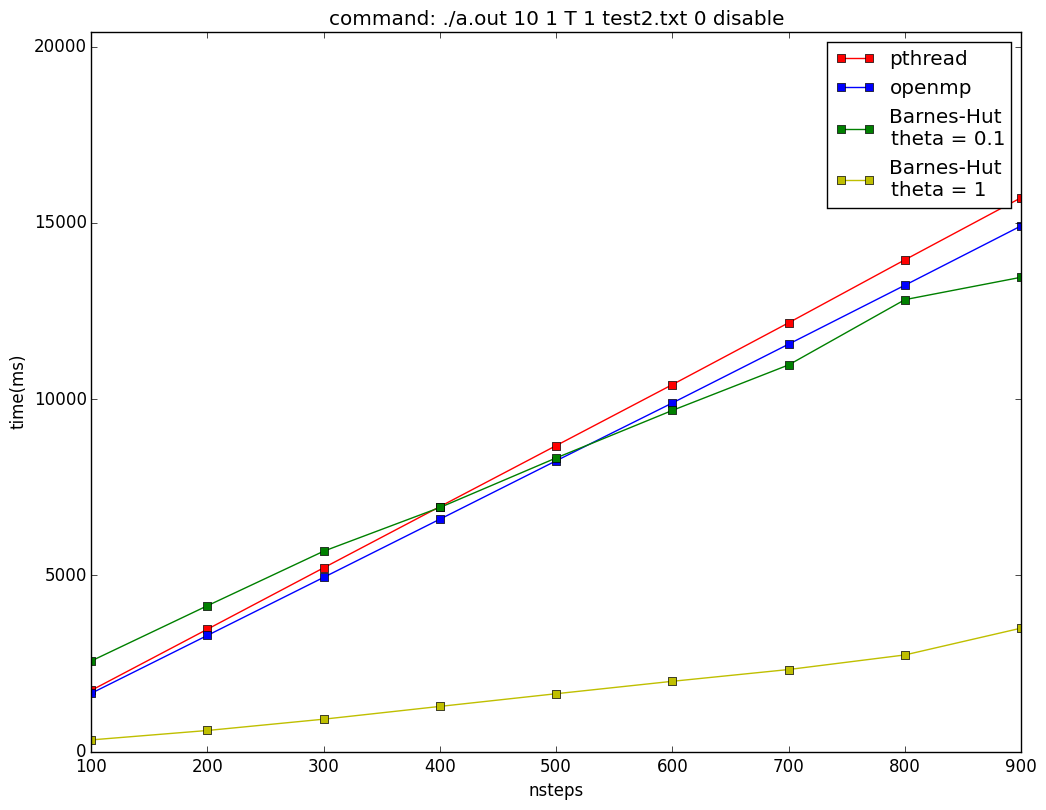
\includegraphics[scale=.5]{./nsteps.png}
				\caption{Results with different number of steps}
			\end{SCfigure}

			\begin{SCfigure}[][h]
				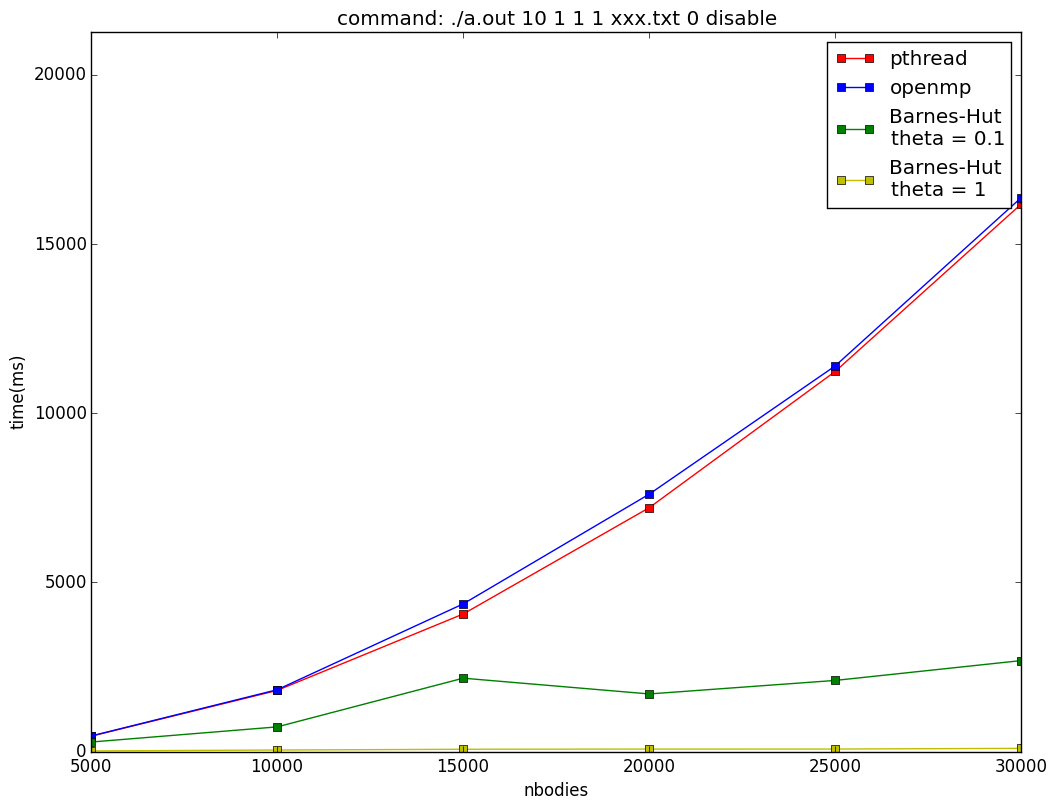
\includegraphics[scale=.5]{./nbodies.png}
				\caption{Results with different number of bodies}
			\end{SCfigure}
		\end{center}

		\newpage

		\item Computation time of Barnes-Hut algorithm
		\begin{SCfigure}[][h]
			\vspace{-80pt}
			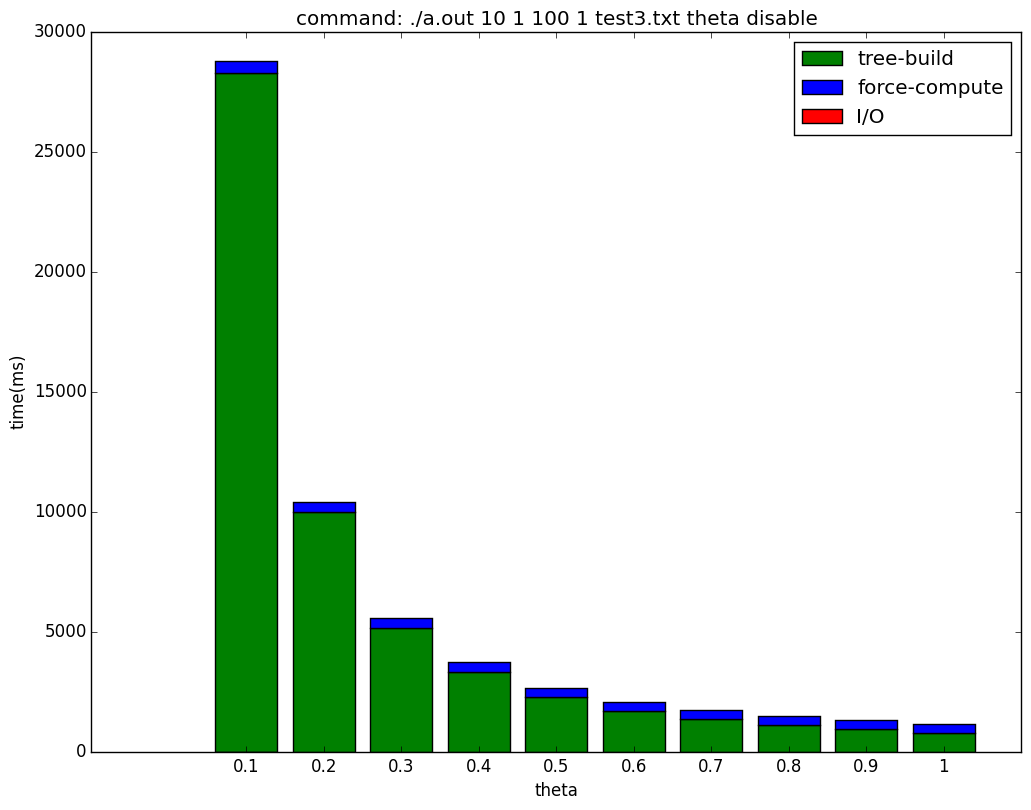
\includegraphics[scale=.5]{./theta.png}
			\caption{Results with different $\theta$}
		\end{SCfigure}
	\end{itemize}
\end{enumerate}

\newpage

\section*{Discussion}
\vspace{-20pt}
\noindent\makebox[\linewidth]{\rule{\textwidth}{0.4pt}}

\begin{enumerate}
	\item Parallelism
	\begin{center}
		\begin{tabular}{|c|c|c|c|}
			\hline
			Type & Complexity & Prop. to ($N_{thread}$ constant) & Prop. to ($N_{body}$ constant) \\
			\hline
			Normal & $O(\frac{N_{body}^2}{N_{thread}})$ & $N_{body}^2$ & $\frac{1}{N_{thread}}$ \\
			\hline
			Barnes-Hut & $O(\frac{N_{body}\log({N_{body}})}{N_{thread}})$ & $N_{body}\log({N_{body})}$ & $\frac{1}{N_{thread}}$ \\
			\hline
		\end{tabular}
	\end{center}
	\begin{flushleft}
		Normal version must compute $N_{thread}^2$ gravitational vectors at each iteration, which grows quadratically as $N_{thread}^2$ increases, regardless of the number of threads used. However, Barnes-Hut algorithm provides an option that allows threads compute gravitational vectors approximately. The larger $\theta$ is, the higher probability that threads go through less bodies occurs, so I simply assume the complexity of using Barnes-Hut algorithm as $O(N_{body}\log(N_{body}))$.
	\end{flushleft}

	\item Perceptual Performance
	\begin{flushleft}
		Using approximation results is similar to computing all pairs at begining, and the visual results will be different as iteration goes. Although there must a difference when using approximation, the results between two methods are roughly the same.
	\end{flushleft}

	\item Things I have learnt
	\begin{flushleft}
		Parallel programming used in scientific computing has many aspects should be concerned, it is inadequate to consider only work-load balanced issue. In the project, I have learnt that memory usage is still an equally important issue that affects the performance very much as well when the number of threads increases. In fact, I have written the project in both C and C++, and finally found C++ version requires so much allocation of the memory that the virtual memory was even allocated and the performance was not improved but worsen consequently. It might be caused by objects with lots of member functions in my design, and the issue was solved when I changed to implement with C. After all, both version of codes will be submitted in case that each of them is needed.
	\end{flushleft}
\end{enumerate}

\end{CJK}
\end{document}